\documentclass[14pt]{article}
\usepackage{allan}
\setlength{\headheight}{60pt}

\lhead{
    \parbox{5cm}{
        \begin{center}
            Problem Chosen \\[0.2cm]
            \textbf{\Huge{A}}
        \end{center}
    }
}
\chead{
    \parbox{5cm}{
        \textbf{
            \begin{center}
                2022 \\
                MCM \\
                Summary Sheet
            \end{center}
        }
    }
}
\rhead{
    \parbox{5cm}{
        \begin{center}
            Team Control Number \\[0.2cm]
            \textbf{\Huge{0000}}
        \end{center}
    }
}
\cfoot{}

\begin{document}
    \begin{center}
        \textbf{\large Summary}
    \end{center}

    This is the summary.

    % real document begins

    %%%%%%%%%%%%%%%%%%%%%%%%%%%%%%%%%%%%%%%%%%%%%%%%%%%%%%%%%%%%%%%%
    \clearpage
    \pagenumbering{arabic}
    \newpage
    \pagestyle{empty}
    \setlength{\headheight}{12pt}
    \renewcommand{\headrulewidth}{0.5pt}
    % \renewcommand{\headrulewidth}{5cm}
    \renewcommand{\footrulewidth}{0.0pt}
    \pagestyle{fancy}
    \lhead{Team \#2226594}
    \chead{Power Profile of a Cyclist}
    \rhead{Page \thepage\ of \pageref{LastPage}}
    \cfoot{}
    \lfoot{}
    \rfoot{}

    %%%%%%%%%%%%%%%%%%%%%%%%%%%%%%%%%%%%%%%%%%%%%%%%%%%%%%%%%%%%%%%%
    \clearpage
    \thispagestyle{empty}
    \tableofcontents
    \newpage
    \pagestyle{fancy}
    \setcounter{page}{1}

	\newpage
	\section{Introduction}
	\subsection{Background}
	Individual time trial is a common type of bicycle road race and has gained popularity in recent years. In individual time trials, individuals will manage to complete their journey on a fixed trial course all by themselves in the shortest possible time and the one that uses the minimum of time seals the victory. 
	
	In cycling activities, each cyclist has a power curve which indicates the maximum power the rider can maintain in the races. Also, given a rider's power curve, cyclists must find the best way to minimize their power usage and maximize their recovering rate. In addition, there are many kinds of individual riders. Common types are time trial specialists, climbers, sprinters, rouleurs and puncheurs. They will act differently when facing various terrains and difficulties. Time trial specialists are good at solving every kinds of problems. The climbers can easily pass the long slopes while puncheurs perform well when facing cliffy slopes. Rouleurs can make good decisions based on different routes. Sprinters have strong explosive force. We will analyze their actions in the following passage.
	
	Moreover, the trial course plays a vital role in the game. It will determine how the cyclists spend their energy and control their speed. It has to be mentioned that all the riders will ride a same course. In games, the condition of trials mostly depends on the type of game and what kind of event it is.
	\subsection{Problem Restatement}
	To make sure that the riders can achieve their best score by using the best strategy (including when to get energy supply and recover) according  to their body condition, we need to find out the relationship between these factors. Therefore, our work is divided into 4 parts:
	\begin{itemize}
		\item  Analyze the power profile of two types if riders given their riding type.
		\item  Build a model calculating their power profile and find out the result when it is applied to different trial courses and various weather conditions. Find out how sensitive the model is.
		\item  Give suggestions to riders and their instructors generally on key turning points after determining how sensitive the model is.
		\item  Extend model so that it can be applied to conditions where a team will take part in a time trial.
	\end{itemize}
	\subsection{General Assumptions}
	\begin{enumerate}
		\item  \textbf{All the dynamic coefficient of friction of the road are equal numbers.}

				To help cyclists achieve better grades and prevent them from serious danger, race organizers usually use artificial tracks. Therefore we can assume that the material of tracks is the same, which means the dynamic coefficient of friction of the road is the same.
		\item  \textbf{All the riders know the terrain of the course and can make their decisions.}
		\item  \textbf{Energies produced by breathing can be stored}
		
				If there is unconsumed energy during the riding process (mainly produced by breathing) , it will be stored. However, it will not exceed the maximum storage amount.
		\item  \textbf{Riders' cycling condition will not change when turning.}
		
				There are not many sharp turns during the game and riders usually spend little time passing them. Therefore we don't take turns into consideration.
		\item \textbf{Riders won't consume any energy when going downhill.}
		
				When riding downhill, riders needn't any energy to keep balance, so we won't consider any speed change when a rider goes downhill.
		\item \textbf{Every rider has an expected completing time.}
			
				According to the second assumption, all the riders know the whole course. Therefore, we can assume that all the cyclists can calculate their expected completing time and their decisions during the game will be affected by this number.
		
	\end{enumerate}
	
	\section{Model A}
	\subsection{Model Overview}
	In the first model, we will discuss the power curve of different types of cyclists. We will discuss the energy consumption of riders according their reactions towards different kinds of terrains and their body conditions. Considering basic energy cost such as breathing and processes of metabolism. We will calculate the power curve based on the maximum power a rider can reach in a certain time and how long he can maintain it. Finally, we will discuss the conditions where basic supplement is needed.
	\subsection{Notation}	
	\begin{tabular}{|l|l|l|}
		\hline
		$\mathrm{T}_\mathrm{exp}$&expected completing time&$\mathrm{s}$\\
		\hline
		$\mathrm{T}_\mathrm{actual}$&actual completing time&$\mathrm{s}$\\
		\hline
		$t$&the time the game lasts for&$\mathrm{s}$\\
		\hline
		$\mathrm{P}(\mathrm{w})$&power of a cyclist&W\\
		\hline
		$\tau(\mathrm{p})$&time which the rider last for at a constant power ($\mathrm{P}(\mathrm{w})$)&$\mathrm{s}$\\
		\hline
		$\mathrm{M}(\mathrm{T})$&the maximum power in the whole process&$\mathrm{W}$\\
		\hline
		$\mathrm{M}(\mathrm{b})$&the maximum power of human body&$\mathrm{W}$\\
		\hline
		$\sigma$&speed of metabolism&$\mathrm{W}$\\ 
		\hline
		$\mathrm{E}_\mathrm{B}$&energy stored before the race&$\mathrm{J}$\\ 
		\hline
		$\mathrm{E}_\mathrm{S}$&energy supplied during the race&$\mathrm{J}$\\ 
		\hline
		$\tau(\mathrm{E}_\mathrm{S})$&time wasted when recovering&$\mathrm{s}$\\ 
		\hline
		$\mathrm{k}$&power restriction index&/\\ 
		\hline
		$\mathrm{m}$&weight of cyclist&$\mathrm{kg}$\\
		\hline
		$f$&air resistance&$\mathrm{N}$\\ 
		\hline
		$\mathrm{v}$&speed of cyclist&m/s\\ 
		\hline
		$\mathrm{C}_\mathrm{D}$&air resistance index&/\\ 
		\hline
		$\rho_\mathrm{air}$&air density&kg/$\mathrm{m}^3$\\ 
		\hline
		$\mathrm{S}_\mathrm{body}$&cyclists' area exposed to air&$\mathrm{m}^2$\\ 
		\hline
		$\mathrm{k}_\mathrm{air}$&air condition index&/\\ 
		\hline
		$D$&distance&m\\
		\hline
		$I$&momentum gathered by wind&$\mathrm{N}$\\ 
		\hline
		$\mathrm{E}_\mathrm{total}$&the total energy stored before the race&$\mathrm{J}$\\ 
		\hline
	\end{tabular}
	\subsection{Calculating Energy Consumption}
	First, we need to consider the cyclist's energy source. We divide a rider's energy consumption into several parts. Considering human's basic physiological activities, energy spent by metabolism needs to be calculated. Therefore we use $\sigma$ to describe human body's speed of metabolism, which is a constant of value 41.5. Moreover, the rider's physical fitness determines his total energy before the race which is defined as $\mathrm{E}_\mathrm{total}$. Finally, cyclists can get energy before the race and energy supplied during the race through food consumption (which we define as $\mathrm{E}_\mathrm{B}$ and $\mathrm{E}_\mathrm{S}$). 

	We use P(t) to desribe the cyclist's power consumption pattern and E(t) to describe the cyclist's energy condition. First we need to figure out how to describe the distance a cyclist has traveled. When a rider is cycling on a plain, what affect his speed and acceleration speed are his power and air resistance (which will be introduced in the next part). There relationship is shown in the picture below:
	\begin{center}
		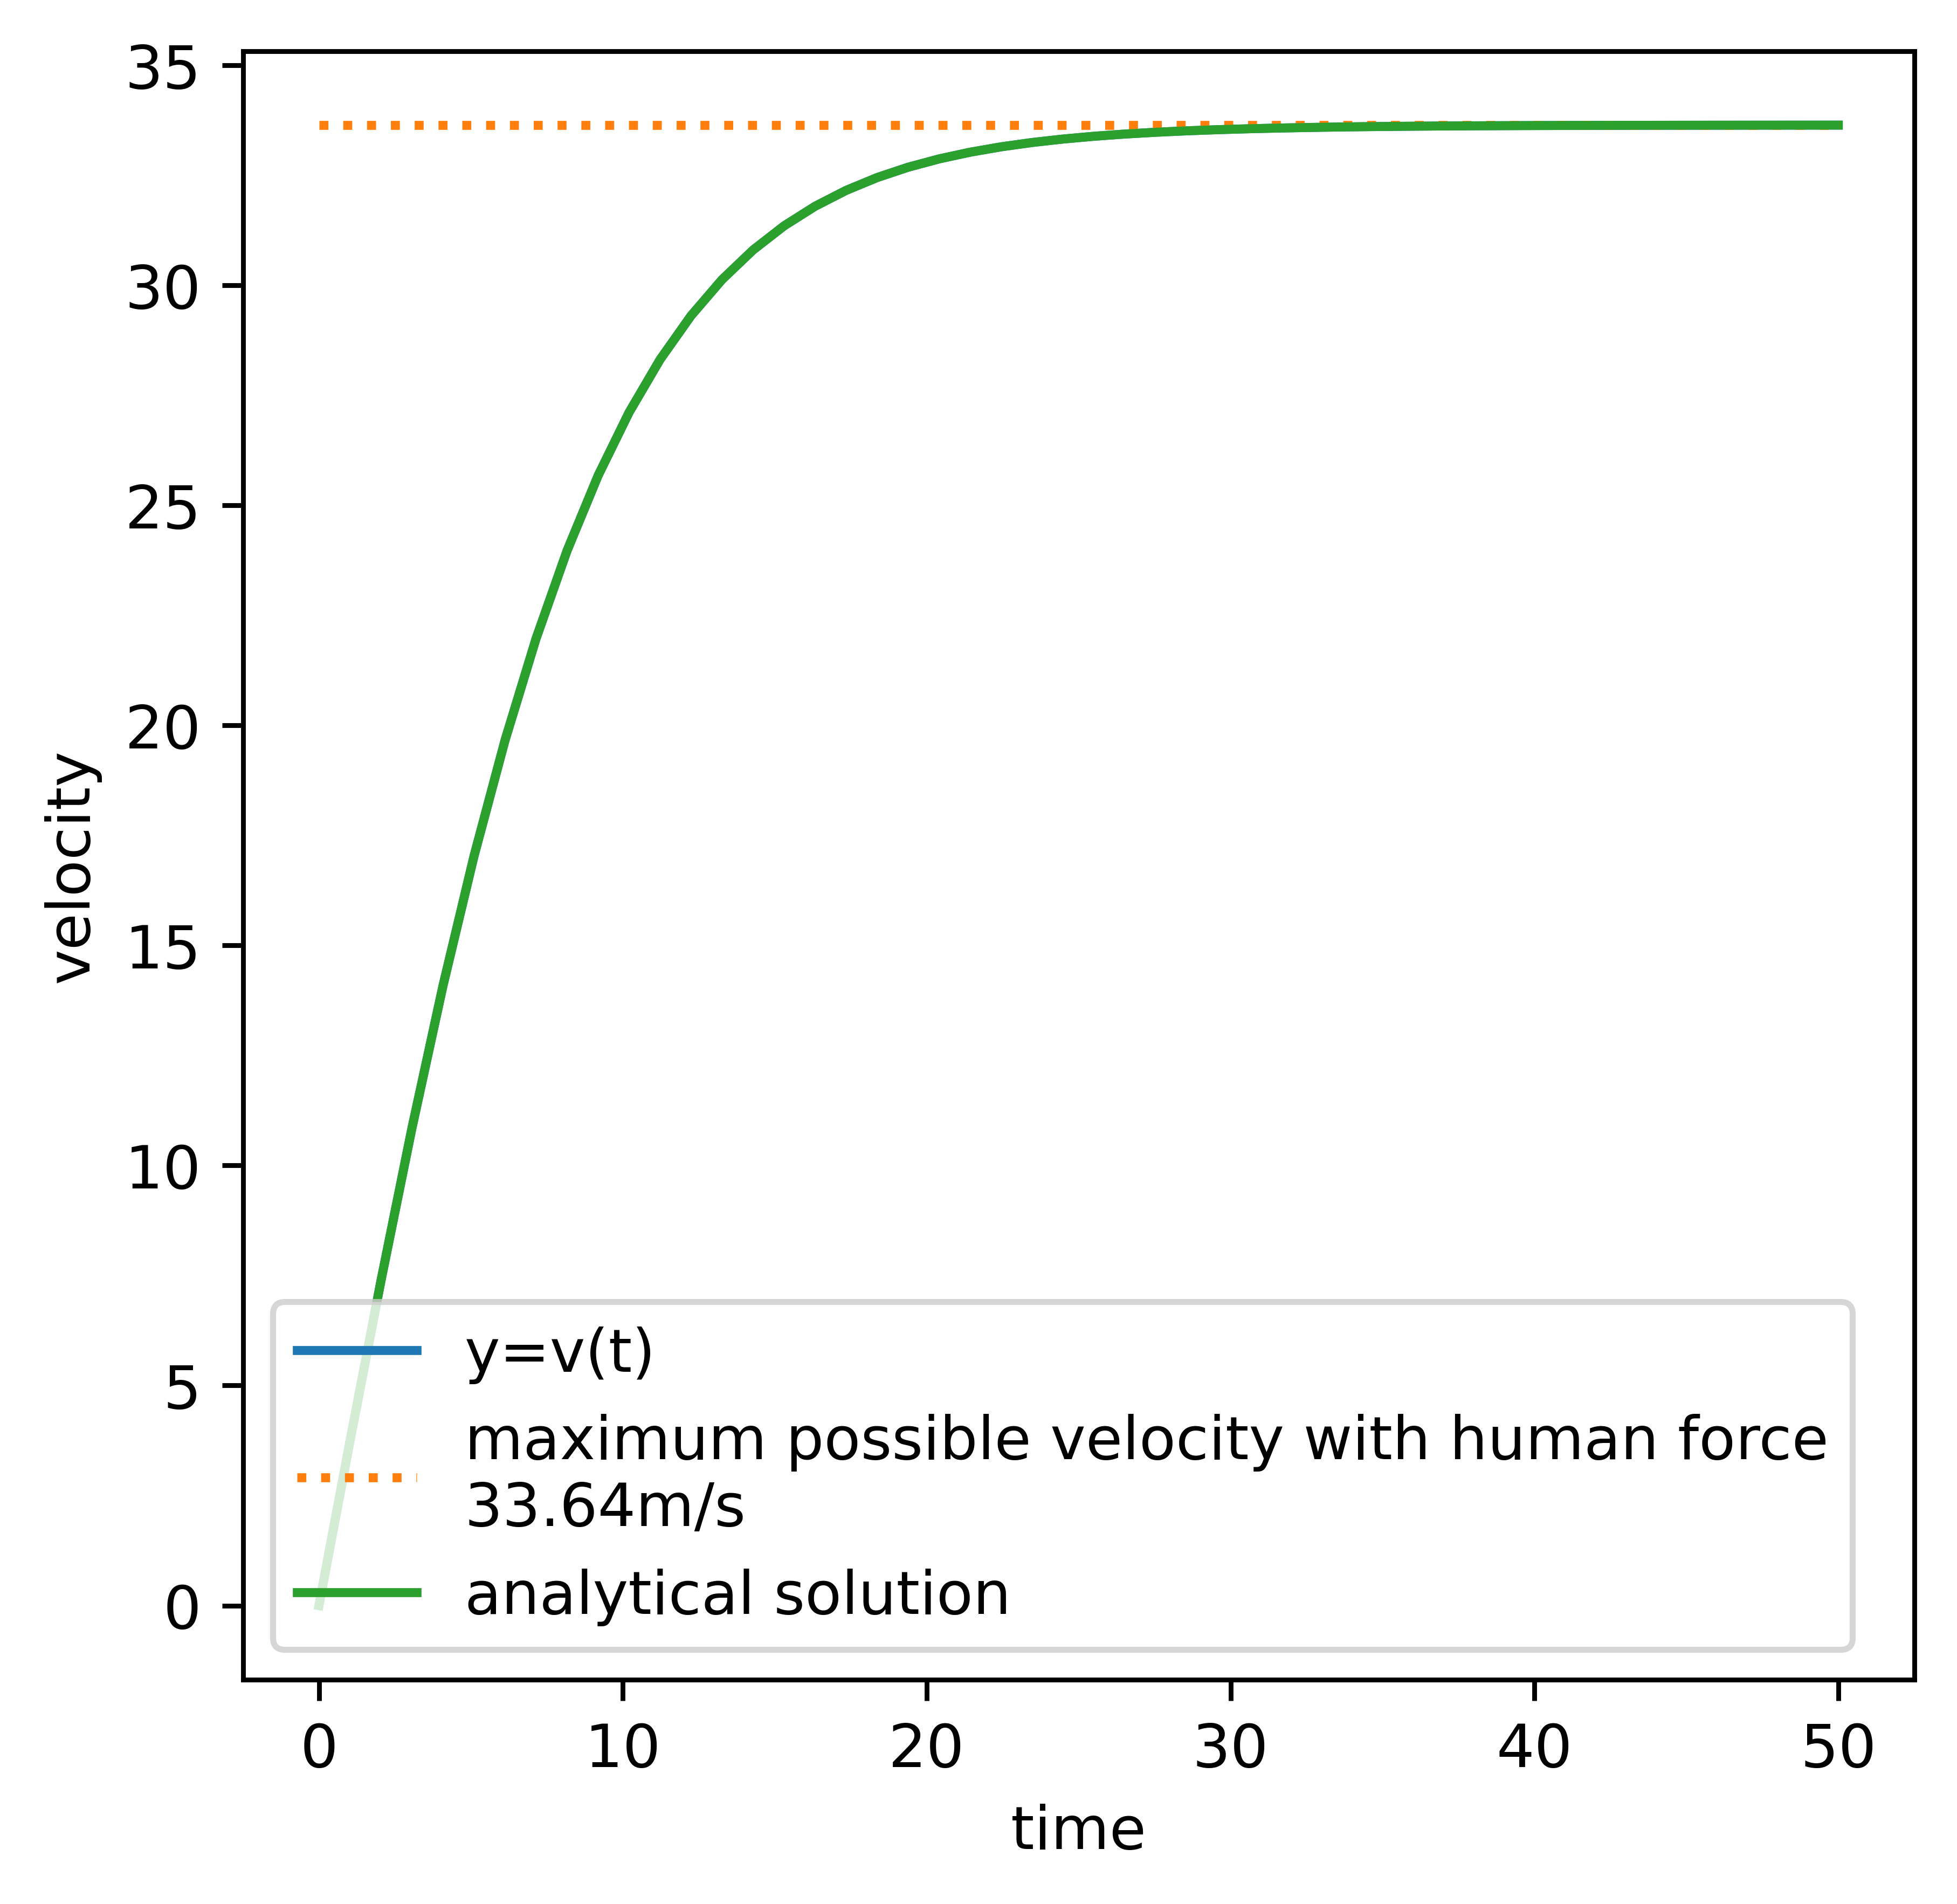
\includegraphics[height=2.5cm]{1.png}

		\small \textit{Fig.1 a cyclist's condition on the plain}
	\end{center}
	 Therefore we can get the following formulae:
	$$D=\int^{\mathrm{T}_\mathrm{actual}}_0 \mathrm{v}(\mathrm{t})\cdot \mathrm{dt}$$
	$$\mathrm{m} \cdot \mathrm{a}(\mathrm{t})=\mathrm{m} \cdot \mathrm{v}\dot(\mathrm{t})=\mathrm{F}-f=\dfrac{\mathrm{P}(\mathrm{t})}{\mathrm{v}}-\dfrac{1}{2}\mathrm{k}\mathrm{v}^2$$
	$$\mathrm{v}(0)=0$$
	$$0\leq\mathrm{P}(\mathrm{t})\leq\mathrm{M}_\mathrm{b}$$
	The second step is to describe the cyclist's condition on the slope. We define $k$ as the index which describes the restriction of power. His condition can be shown in the picture below:
	\begin{center}
		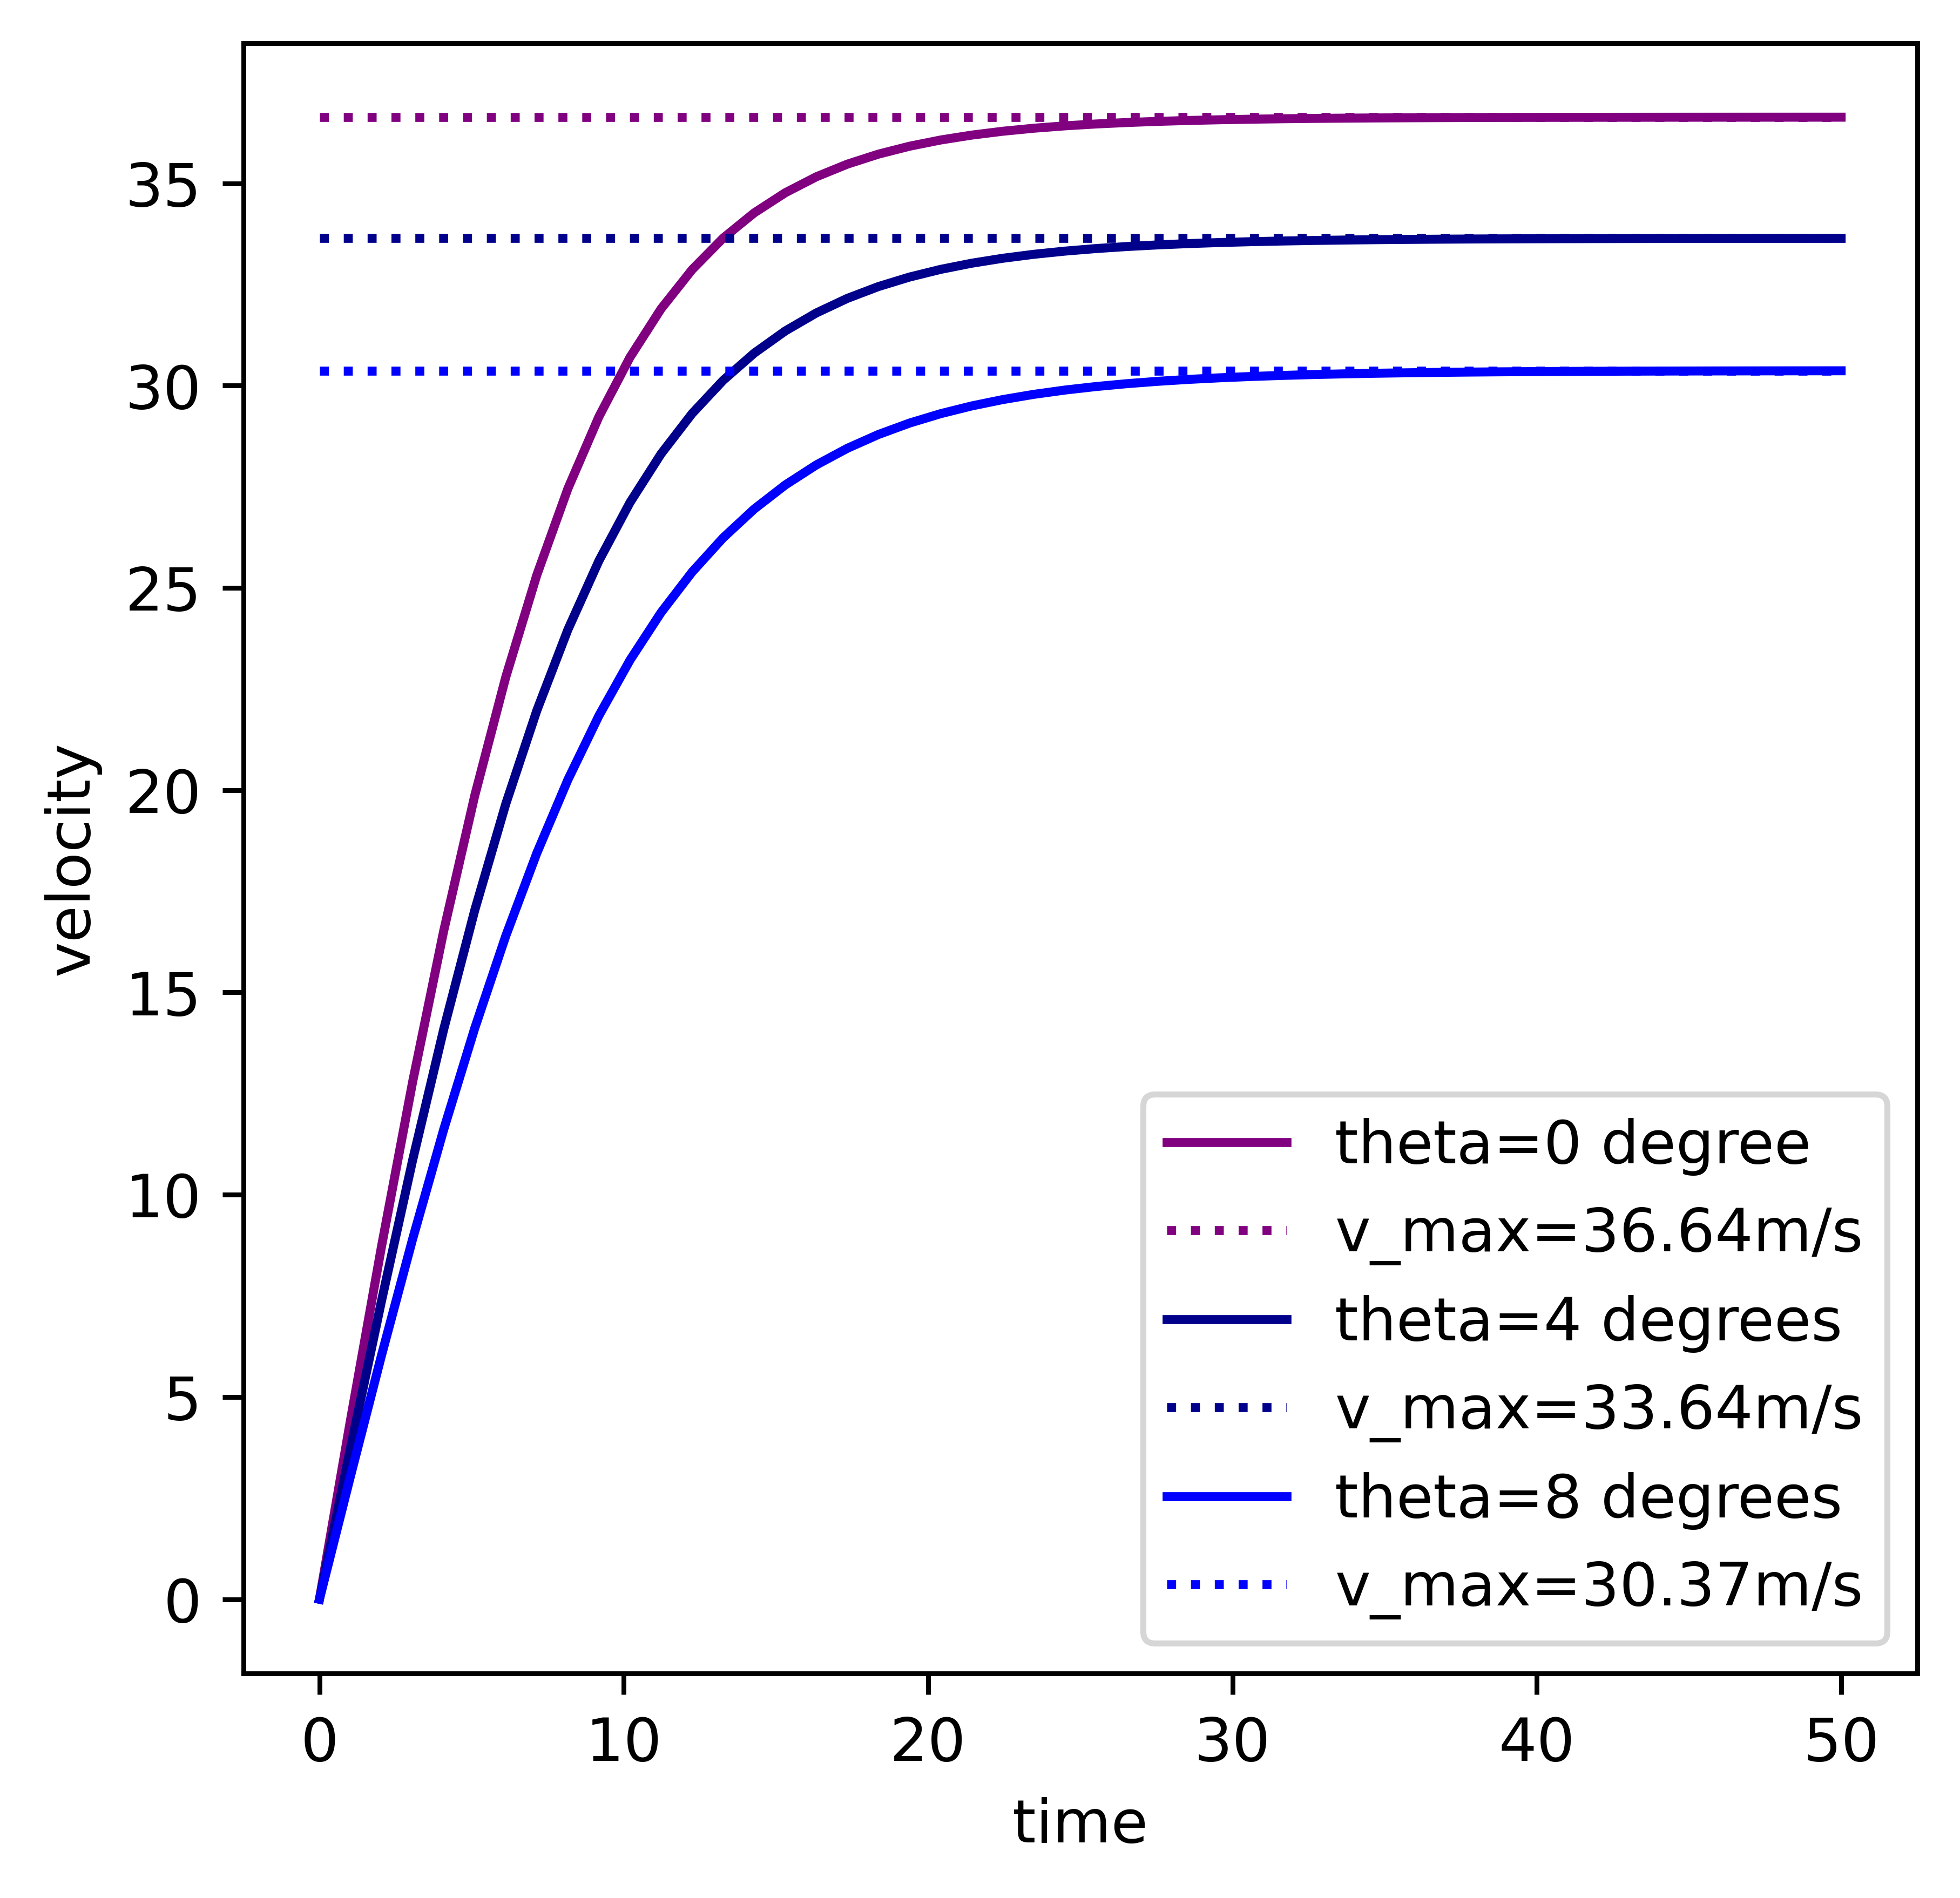
\includegraphics[width=7cm]{2.png}

		\small \textit{Fig.2 a cyclist's condition on the slope}
	\end{center}
	Under this circumstance, if $\mathrm{P}(\mathrm{t}) \ge \mathrm{M}$, his power pattern can be calculated through the formulae below:
	$$\mathrm{P}\dot(\mathrm{t})=-\dfrac{1}{\mathrm{k}} \mathrm{P}(\mathrm{t}) \cdot \dfrac{1}{\mathrm{E}(\mathrm{t})}$$
	$$\mathrm{E}\dot(\mathrm{t})=\sigma-\left(f+mg\sin\theta+\mu mg\cos \theta\right)\cdot \mathrm{v}
	(\mathrm{t})$$
	$$\mathrm{E}(0)=\mathrm{E}_\mathrm{total}$$
	$$\mathrm{E}(\mathrm{t})\geq0, \forall 0 \leq \mathrm{t} \leq \mathrm{T}_\mathrm{total}$$
	$$\mathrm{E}(\mathrm{t})=\left[\sigma-\left(f+mg\sin \theta +\mu mg \cos \theta \right)\cdot \mathrm{v}(\mathrm{t})\right]\cdot \mathrm{t}+\mathrm{E}_\mathrm{total}$$
	$$\mathrm{E}(\mathrm{t})=-\dfrac{\mathrm{P}(\mathrm{t})}{\mathrm{k}\cdot \mathrm{P}\dot(\mathrm{t})}=-\dfrac{\mathrm{m}\mathrm{v}\ddot(\mathrm{t})+\dfrac{1}{2}\mathrm{k}{\mathrm{v}(\mathrm{t})}^3}{\mathrm{m}\mathrm{v}\dot(\mathrm{t})\cdot\mathrm{v}(\mathrm{t})+\mathrm{v}\dot(\mathrm{t})^2+\dfrac{3}{2}\mathrm{k}{\mathrm{v}(\mathrm{t})}^2}$$
	By calculating the energy cost, we can also get the relationship between the cyclist's power usage and his speed and his weight,which is:
	$$\mathrm{P}(\mathrm{t})=\mathrm{m}\mathrm{v}\dot(\mathrm{t})\cdot \mathrm{v}(\mathrm{t})+\dfrac{1}{2}\mathrm{k}{\mathrm{v}(\mathrm{t})}^3$$
	$$\mathrm{P}\dot(\mathrm{t})=\mathrm{m}\mathrm{v}\ddot(\mathrm{t})\mathrm{v}(\mathrm{t})+{\mathrm{v}\dot(\mathrm{t})}^2+\dfrac{3}{2}\mathrm{k}{\mathrm{v}(\mathrm{t})}^2$$
	\subsection{Calcucaling Air Resistance}
	Since the cyclists will race against each other in a quick speed, the air resistance ($f$) can't be neglected. We define $f$ as the formulae follow:
	$$f=\dfrac{1}{2} \mathrm{C}_\mathrm{D} \cdot \rho_\mathrm{air} \mathrm{S}_\mathrm{body} v^2$$
	$$\mathrm{k}_\mathrm{air}=\dfrac{1}{2} \mathrm{C}_\mathrm{D} \rho_\mathrm{air}$$
	$$f=\mathrm{k}_\mathrm{air}\cdot \mathrm{v}^2$$
	After searching related data from academic literature, we find out that $\mathrm{C}_\mathrm{D}=0.024$, $\rho_\mathrm{air}=1.293 \mathrm{kg/}\mathrm{m}^3$ and $\mathrm{S}_\mathrm{body}=0.209 \mathrm{m}^2$. Based on these data, we can indicate that $\mathrm{k}_\mathrm{air}\approx0.0032$.
	%\newpage
	\section{Model B}
	\subsection{Model Overview}
	In this model, we will firstly discuss how to descibe rider's basic feature and their power curve in detail. Later, we will also take special factors such as climate ino consideration. Finally, we will apply our model into several distinct trial courses and get out the answer.
	\subsection{Assumptions}
	\begin{enumerate}
		\item	\textbf{Rain is not considered in this model.}

				Many activities have been cancelled or delayed because of rainy days in the past few years. But if the trial's humidity is under the criteria. Roads' dynamic coefficient of friction won't be affected.
	\end{enumerate}
	\subsection{Notation}
	\begin{tabular}{|l|l|l|}
		\hline
		$\mathrm{m}(\mathrm{x})$&weight of cyclist&$\mathrm{kg}$\\
		\hline
		$\mathrm{h}(\mathrm{x})$&height of cyclist&$\mathrm{m}$\\
		\hline
		$\mathrm{BMI}(\mathrm{x})$&body mass index of cyclist&/\\
		\hline
		$\mathrm{E}_\mathrm{total} (\mathrm{x})$&total energy of cyclist&$\mathrm{J}$\\
		\hline
		$\mathrm{S}_\mathrm{body}(\mathrm{x})$&body measure&$\mathrm{m}^2$\\
		\hline
		$\mathrm{T}_\mathrm{min}$&the least time spent to complete the game&$\mathrm{s}$\\
		\hline
		$\mathrm{F}_\mathrm{wind}$&wind force&$\mathrm{N}$\\
		\hline
		$\mathrm{T}$&temperature of the trial&$\circ$\\
		\hline
	\end{tabular}
	\subsection{Calculate Total Energy}
	In this part, we will mainly discuss the cyclist's total power based on his phisycal condition and cycling type. 

	First, we need to have a basic understanding of the cyclist's physical condition. Take Tour de France as an example\cite{france}. Among the champions of this race in the past five years, their average height is 1.808$\mathrm{m}$ and their average weight is 68.58$\mathrm{kg}$. Olympic cyclists have an average height og 1.80$\mathrm{m}$ and an average of around 68$\mathrm{kg}$\cite{weight}. 

	In our model, we use a series of variables with (x) to describe the cyclist's features. These include $\mathrm{m}(\mathrm{x})$, $\mathrm{h}(\mathrm{x})$, etc. According to the BMI criteria, we can get the formula:
	$$\mathrm{BMI}(\mathrm{x})=\dfrac{\mathrm{x}}{\mathrm{h}^2(\mathrm{x})}$$
	Also, since where our body is exposed to air can be seen as a square, we can find that:
	$$\mathrm{S}_\mathrm{body}(\mathrm{x})\propto\mathrm{h}^2(\mathrm{x})$$
	\subsection{Weather Conditions}
	There are many factors that will affect the speed. They are temperature and wind force. 
	\subsubsection{Temperature}
	\subsubsection{Wind force}
	\subsection{Recalculate Speed Function}
	After we have discussed the weather's impact on our model, we need to polish it so that it can be applied to special cases as well. Considering that there is no air resistance but wind force now, we need to recalculate the speed function.

	If the momentum is a constant number (which we define as $\mathrm{F}(\mathrm{t})$), we can get the following formulae:
	$$\mathrm{m}\mathrm{v}\dot(\mathrm{t})=\mathrm{F}(\mathrm{t})-f-\mathrm{F}_{f}-mg\sin \theta=\mathrm{F}(\mathrm{t})-\mathrm{k}_\mathrm{air}{\mathrm{v}(\mathrm{t})}^2-\dfrac{mg\mu}{\mathrm{r}_\mathrm{wheel}}-mg\sin \theta$$
	$$\mathrm{v}(0)=0$$
	$$0\leq\mathrm{F}(\mathrm{t})\leq\mathrm{F}_\mathrm{m}$$
	, and:
	$$\mathrm{E}\dot(\mathrm{t})=\sigma-\mathrm{F}(\mathrm{t})\cdot\mathrm{v}(\mathrm{t})$$
	$$\mathrm{E}(0)=\mathrm{E}_\mathrm{total}$$
	$$\mathrm{E}(\mathrm{t})\geq0$$
	beiyong
	
	$\mathrm{A}=\mathrm{F}_\mathrm{m}-\dfrac{mg\mu}{\mathrm{r}_\mathrm{wheel}}-mg\sin \theta$

	$\mathrm{v}(\mathrm{t})\\=\\\dfrac{\sqrt{\mathrm{F}_\mathrm{m}-\dfrac{mg\mu}{\mathrm{r}_\mathrm{wheel}}-mg\sin \theta} \tan \mathrm{h} \left(\dfrac{\sqrt{\mathrm{F}_\mathrm{m}-\dfrac{mg\mu}{\mathrm{r}_\mathrm{wheel}}-mg\sin \theta}\ \ \mathrm{C}\sqrt{\mathrm{k}_\mathrm{air}} m+\sqrt{\mathrm{F}_\mathrm{m}-\dfrac{mg\mu}{\mathrm{r}_\mathrm{wheel}}-mg\sin \theta}\ \ \sqrt{\mathrm{k}_\mathrm{air}} x}{\mathrm{m}}\right)}{\sqrt{\mathrm{k}_\mathrm{air}}}$

	$=\dfrac{\sqrt{\mathrm{A}} \tan \mathrm{h}\left[\dfrac{\left(\mathrm{m}\mathrm{C}_1+\mathrm{x}\right)\sqrt{\mathrm{Ak}}}{\mathrm{m}}\right]}{\sqrt{\mathrm{k}}}$

	$\mathrm{v}(0)=\dfrac{\sqrt{\mathrm{A}} \tan h \left(\mathrm{C}_1\sqrt{\mathrm{Ak}}\right)}{\sqrt{\mathrm{k}}}$

	By doing this we can get the result: $\mathrm{C}_1=0$
	\section{Strengths and Weaknesses}
	\subsection*{Strengths}
	\begin{itemize}
		\item
	\end{itemize}
	\subsection*{Weaknesses}
	\begin{itemize}
		\item 
	\end{itemize}
	\newpage
	\thispagestyle{empty}
	% \setcounter{page}{\wholepages}
	\renewcommand\refname{References}
	\clearpage
	\addcontentsline{toc}{section}{References}
	\tolerance=500
	\begin{thebibliography}{100}
		\bibitem{114514} Math Modelling, Qiyuan Kang, Jinxing Xie and Jun YeMath Modelling
		\bibitem{UCI}2021 Road World Championships Individual Time Trial (Men Elite), UCI,
		
		https://www.flanders2021.com/\_media/races/image\_map/1632122636/fit/1650/0/6/men-elite-individual-time-trial.webp
		\bibitem{france}https://www.topendsports.com/sport/cycling/anthropometry-tourdefrance-tables.htm
		\bibitem{weight}Cycling Physique, science4performance,
		
		https://science4performance.com/2019/09/12/cycling-physique/
		\bibitem{friction}https://zhidao.baidu.com/question/309300297713546924.html
	\end{thebibliography} 
	
\end{document}
